\documentclass{article}

\usepackage{arxiv}

\usepackage[utf8]{inputenc} % allow utf-8 input
\usepackage[T1]{fontenc}    % use 8-bit T1 fonts
\usepackage{hyperref}       % hyperlinks
\usepackage{url}            % simple URL typesetting
\usepackage{booktabs}       % professional-quality tables
\usepackage{amsfonts}       % blackboard math symbols
\usepackage{nicefrac}       % compact symbols for 1/2, etc.
\usepackage{microtype}      % microtypography
\usepackage{cleveref}       % smart cross-referencing
\usepackage{graphicx}
\usepackage{natbib}
\usepackage{doi}
\usepackage{csquotes}
\usepackage{enumitem}
\usepackage{tabularx}
\usepackage{tikz}
\usepackage{pgfplots}
\usepackage[normalem]{ulem}
\pgfplotsset{compat=1.18}

\usetikzlibrary{matrix,positioning,fit,shapes.geometric,arrows.meta}

\title{Knowledge Markers: An AI-Agnostic Concept for the Design of Programming Courses}


\newif\ifuniqueAffiliation
% Comment to use multiple affiliations variant of author block 
\uniqueAffiliationtrue

\ifuniqueAffiliation % Standard variant of author block
\author{ \href{https://orcid.org/0000-0003-1686-3460}{
\includegraphics[scale=0.06]{orcid.pdf}\hspace{1mm}Christina Maria Mayr}\thanks{
		\href{https://christinamaria-mayr.userweb.mwn.de/}{christinamariamayr.de}} \\
		Department of Mechanical, Automotive and Aeronautical Engineering\\
	Hochschule München University of Applied Sciences\\
	Germany, Munich \\
	\texttt{christina\_maria.mayr@hm.edu} \\
	%% examples of more authors
}
\else
% Multiple affiliations variant of author block
\usepackage{authblk}
\renewcommand\Authfont{\bfseries}
\setlength{\affilsep}{0em}
% box is needed for correct spacing with authblk
\newbox{\orcid}\sbox{\orcid}{
\includegraphics[scale=0.06]{orcid.pdf}} 
\author[1]{%
	\href{https://orcid.org/0000-0003-1686-3460}{\usebox{\orcid}\hspace{1mm}Christina Maria Mayr\thanks{\texttt{christina\_maria.mayr@hm.edu}, \url{christinamariamayr.de}}}%
}
\affil[1]{Department of Mechanical, Automotive and Aeronautical Engineering, Hochschule München University of Applied Sciences, Munich, Germany}
\fi

% Uncomment to override  the `A preprint' in the header
%\renewcommand{\headeright}{Technical Report}
%\renewcommand{\undertitle}{Technical Report}
\renewcommand{\shorttitle}{Knowledge Markers for Course Design}

%%% Add PDF metadata to help others organize their library
%%% Once the PDF is generated, you can check the metadata with
%%% $ pdfinfo template.pdf
\hypersetup{
pdftitle={Knowledge Markers: An AI-Agnostic Concept for the Design of Programming Courses},
pdfsubject={Software engineering education, generative AI, course design},
pdfauthor={Christina Maria Mayr},
pdfkeywords={software engineering education, generative AI, programming education, learning materials, open educational resources},
}

\begin{document}
\maketitle

\begin{abstract}
Generative AI allows students to produce plausible code quickly. 
Producing working code is therefore no longer a reliable indicator of understanding. This matters especially in non-computer-science programmes. In these courses, time is limited, and instructors must decide which contents still serve learning when implementation can be partly automated.
%
This paper contributes knowledge markers as a simple, AI-agnostic concept for programming course design. The markers label learning units by their main knowledge demand: (A) Application knowledge (implementation), (S) Structure knowledge (concepts and mental models), or (P) Procedure knowledge (systematic methods, decision making, and verification). They connect learning theory to concrete teaching materials and make learning intent visible for instructors, students, and later analysis.
We show how the markers can be assigned manually with a decision process. We also show how large language models can generate independent label proposals for consistency checks. 
We demonstrate the approach in a descriptive course-design case: we analyse existing material, redesign an introductory programming course for a non-computer-science programme, embed the labels in open teaching artifacts, and summarise the resulting course structure with marker distributions. 
By making knowledge demands explicit, the markers help instructors assess whether course contents still contribute to learning in the age of LLMs. 
They also help students choose suitable learning strategies and make AI-related studies in programming education easier to compare.
\end{abstract}


% keywords can be removed
\keywords{software engineering education \and generative AI \and programming education \and open learning materials \and verification}

\section{Introduction}

The availability of generative artificial intelligence changes what it means to learn programming. Tasks that once required detailed knowledge of syntax and implementation can now be completed with little effort using large language models. As a result, producing working code is no longer a reliable indicator of understanding.

This raises a central question for programming education:
\textit{What does it mean to learn programming when solution production becomes cheap?}
If students can generate plausible solutions without understanding them, then observable performance and actual learning can diverge. 
Empirical results point in this direction. \citet{BassnerEtAl2026LessStress} found that tool support improved task scores and reduced frustration, but did not improve learning gains or code-comprehension skills. 
Weak understanding in introductory programming is not new, but easy code generation makes it harder to detect. 
\citet{ListerEtAl2004Tracing} show that this problem existed before generative AI. In their multi-national study, many students at the conclusion of their introductory programming course still could not reliably read and trace short programs. In other words, reaching the end of the course did not necessarily mean that core programming understanding had been learned. Huihui et al.~\citet{HuihuiQiPhan2023} argue that students do not necessarily learn concepts deeply by solving problems, unless they reflect their doing before and during the task. Also, they advocate for oral exams to better understand students reasoning behavior.
 

Instructors therefore face several choices when integrating AI into teaching. A course may prohibit AI use, allow it as an optional assistant, integrate an AI tutor, or let students use a general-purpose model as a code generator. Studies already compare some of these options. For example, \citet{BassnerEtAl2026LessStress,bassner2025understanding} compared settings in which students worked without tool support, with the AI tutor IRIS \citep{bassner2024iris}, or with a general-purpose large language model that can also generate code. These conditions mirror common teaching choices: no AI support, AI as a tutor or assistant, and AI as a code generator.

The difficulty is that these studies lead to different and context-dependent results. 
\citet{BassnerEtAl2026LessStress,bassner2025understanding} show in the same teaching context that the evaluation of AI support depends on the assessment criterion. AI support appears beneficial when task scores or frustration are measured, but not when learning gains or code-comprehension skills are measured. Other studies use further criteria and report different patterns. 
For example, \citet{jost-2024-impact-llms-programming-education} reported lower final grades when students relied more on large language models for tasks that require critical thinking, such as code generation and debugging. 
In contrast, \citet{math12050629} reported no clear performance differences associated with ChatGPT use in their setting.
Beyond these performance results, \citet{Qian2025PedagogicalGenAIHE} identify a broader pedagogical risk in their review of generative AI in higher education: students may outsource cognitive and metacognitive work to AI systems.

This makes the findings difficult to translate into course design. Studies use different tools, tasks, policies, cohorts, and outcome measures. Some are conducted in computer science programmes, while others address programming in non-computer-science or vocational contexts, where time constraints, student motivation, and prior knowledge can differ. 
Review work has begun to compare and organise this heterogeneous evidence. For example, \citet{RaihanEtAl2025LLMCSeduSLR} summarise studies across use cases and tools. Such reviews show contradictory findings, but they do not yet evaluate what these contradictions mean for concrete teaching decisions. They also do not provide concrete course-level recommendations. Instructors still have to decide for themselves which contents should be changed, protected, moved to self-study, or redesigned when AI tools are available.\par

At the same time, educational theory offers useful concepts for understanding learning, but it can be difficult to apply them in everyday teaching. Theories describe types of knowledge \citep{Krathwohl2002} and cognitive processes such as cognitive load \citep{SwellerAyresKalyuga2011CognitiveLoadTheory}. Evidence syntheses also highlight that practice-oriented translation into instructor-ready guidance is often missing \citep{ZawackiRichterEtAl2019Educators}. In the era of code-generating tools, this matters because writing code can look like competence even when understanding is weak. The challenge is especially strong for instructors without formal didactic training, who must make practical decisions under time and curriculum constraints.\par

We conclude that the core problem is an operational gap between evidence, theory, and course design. Empirical AI studies often describe local outcomes for one tool, task, or cohort. Learning theory describes knowledge types and cognitive processes, but it is often too abstract to guide decisions about concrete course units. Guidance documents stress the need for appropriate AI use in education, but they usually remain at a high level; see, for example, \citep{UNESCO2023GenAI}. What remains missing is a usable middle layer: a way to translate learning intentions into concrete teaching structures and AI-use decisions for instructors and learners.\par

In this paper, we address this gap by introducing a practical, theory-informed concept for structuring programming education: \emph{knowledge markers}. The markers label learning units according to three complementary knowledge emphases—(A) Application knowledge, (S) Structure knowledge, and (P) Procedure knowledge. The concept is independent of specific tools and can be applied in teaching settings with and without AI. 
It does not prescribe whether AI should be used. Instead, it makes the intended learning demand explicit. This is necessary before instructors can judge where AI may help, where it may hide missing understanding, and where its use should be restricted or guided. It is also necessary for reproducible AI studies in programming education: without a clear description of the knowledge demand of a task or course unit, it remains unclear what an AI intervention was intended to affect.


The paper makes the following contributions:
\begin{itemize}[leftmargin=*]
\item \textbf{A theory-informed, AI-agnostic structuring concept:}
We introduce the A/S/P knowledge markers as a practical concept for structuring programming education, independent of specific tools and applicable both with and without AI.
\item \textbf{Course analysis under LLM conditions:}
The markers make it possible to analyse existing and redesigned course contents with respect to their knowledge demands and their role in an environment where implementation can be partly automated.
\item \textbf{Enabling targeted AI use through explicit labels:}
The markers make learning goals explicit and provide guidance for how AI can be used depending on the targeted knowledge type, thereby translating abstract learning theory into concrete teaching decisions.
\item \textbf{Accessibility for non-didactic experts:}
The concept gives instructors and students a simple way to structure and reflect on learning activities without specialised pedagogical expertise.
\item \textbf{Manual and LLM-supported assignment:}
We show how human raters can assign markers with a decision process. We also show how LLMs can generate independent label proposals for reflection and consistency checks.
\item \textbf{Application in software education:}
We demonstrate the approach in a real programming course through a descriptive course-design case and provide openly available learning artifacts to support adoption.
\end{itemize}

The remainder of this paper is structured as follows. \Cref{sec:related-work} reviews related work on AI-supported programming education and relevant learning theory. \Cref{sec:asv} introduces the knowledge markers and the underlying concept. The subsequent section describes their implementation and use in a course setting. The paper concludes with implications for AI-supported teaching and directions for future work.

\section{Related Work}
\label{sec:related-work}
This section reviews work that motivates a simple course-level concept for structuring learning with generative artificial intelligence.
We first review studies on unstructured use of generative AI in programming education. These studies show that students can produce working code while learning outcomes remain unclear or weak. We then review studies that embed generative AI into designed learning activities. These studies show that learning depends on activity design choices such as scaffolds (prompts, intermediate steps, constraints, or explanation requirements) and other guardrails. We also review work on tutoring systems. Such systems can work well in one setup, but they are hard to transfer across courses. Finally, we summarise learning theory and novice cognition to clarify what course design must protect and train.

\subsection{Usage of generative artificial intelligence in novice programming education}
Raihan et al.\ conducted a systematic literature review on large language models in computer science education \citep{RaihanEtAl2025LLMCSeduSLR}. Across the surveyed studies, they report use in diverse educational contexts, while evidence about learning gains remains mixed.\par
\citet{RozputniaEtAl2025AISupportVocationalProgramming} discuss AI as a support tool for programming education in vocational bachelor's programmes. They describe adaptive learning systems, intelligent tutoring systems, automated code evaluation, and generative models as possible uses. They also identify academic-integrity risks, especially when students generate solutions without understanding the subject matter.
Kazemitabaar et al.\ ran a controlled study with novice learners using an AI code generator for introductory Python tasks \citep{KazemitabaarEtAl2023AICodeGenerators}. They found higher completion and higher task scores, and they did not find worse follow-up results on unaided tasks in their setting.
Bassner et al.\ conducted a study in which students solved a programming task in three settings: without AI, with the AI tutor IRIS \citep{bassner2024iris}, and with a general-purpose LLM \citep{BassnerEtAl2026LessStress}. IRIS gives advice but does not reveal the solution. The authors report better exercise scores in the two AI groups and less frustration. They do not find higher learning gains or better comprehension. In related work, \citet{frankford2024aitutoring} state that AI tutors can help scale support to large cohorts, but they also describe concerns about generic responses and overreliance.
%
Sankaranarayanan \citep{Sankaranarayanan2026EpistemicDebt} observed two novice behaviours in AI-supported programming: a \emph{contractor} stance that outsources work to the model and a \emph{consultant} stance that treats it as a partner and asks for explanations. They also tested how well novices can identify and fix a race condition when AI support is suddenly turned off in the Cursor IDE. In the group without AI access, 18/26 students succeeded (69.2\%). In the AI group where students could use AI only after explaining their intentions, 16/26 succeeded (61.5\%). In the group with unsupervised AI use, 6/26 succeeded (23.1\%). These findings show that students can use AI to complete tasks while still lacking transferable debugging ability.
%
Denny et al.\ investigated how to evaluate and enhance code comprehension \citep{DennyEtAl2024EiPE}. Their approach has students explain code in plain English, supported by a large language model.
Ma et al.\ introduce Decomposition Box (DBox), an interactive LLM-based system that helps learners break problems into structured steps \citep{MaEtAl2025DBox}. The system and the learner jointly construct a step-by-step solution process. The system adapts its level of help based on the learner's progress. In a within-subjects study (N=24), the authors report improvements in learning gains, cognitive engagement, and critical thinking compared to a baseline condition.
Liffiton et al.\ introduced CodeHelp, an LLM tool that provides assistance to programming students without directly revealing solutions \citep{LiffitonEtAl2023CodeHelp}. The authors report that the tool is well-received, leaving open whether it enhances understanding or improves performance.
Jacobs and Jaschke designed a web application that uses GPT-4 to provide feedback on programming tasks without revealing the solution \citep{JacobsJaschke2024LLMFeedback}.
%
Kuhail et al.\ conducted a systematic review on educational chatbots \citep{KuhailEtAl2023EducationalChatbotsSLR}. They identify recurring design and evaluation limitations and a lack of consistent, instructor-ready guidance.
%
Dermeval et al.\ reviewed authoring tools for intelligent tutoring systems and show that development and adaptation remain costly \citep{DermevalEtAl2018ITSAuthoringToolsSLR}. Schiff discusses challenges when moving educational AI from prototypes into classrooms and highlights socio-technical constraints that make transfer difficult \citep{Schiff2021OutOfLab}.

These studies show that students can produce working code with AI support. They also show that learning depends on how tool use is structured and on what learners must explain and verify. What remains open for everyday teaching is a simple, transferable way to state the learning intent of each unit. This is needed so that generative AI supports learning rather than only task performance. To address this limitation, we now turn to learning theory and evidence on novice cognition.\par

\subsection{Learning theory and novice cognition}
Several learning theories are relevant here, including cognitive approaches \citep{NRC1999HowPeopleLearn}, constructivism \citep{Glasersfeld1989Constructivism}, and social learning theory \citep{Bandura1977SocialLearning}. These theories describe important learning mechanisms. However, they operate at a high level of abstraction. They do not directly specify how instructors should structure learning activities, especially in AI-supported settings.

One relevant distinction is between types of knowledge. Krathwohl distinguishes, for example, between factual, conceptual, procedural, and metacognitive knowledge \citep{Krathwohl2002}. In programming, this corresponds to knowing syntax, understanding program structure, being able to apply solution procedures, and reflecting on one's own reasoning. This distinction clarifies what kinds of knowledge are involved, but it does not indicate how learning activities should be structured when tools can generate code.
%
Cognitive load theory highlights that working memory is limited and that learning tasks must be designed carefully to avoid overload \citep{SwellerAyresKalyuga2011CognitiveLoadTheory}. When AI reduces the effort required for code production, it can also shift cognitive effort away from essential processes such as reasoning about program behaviour. This raises the question of how tasks should be structured so that reduced effort does not lead to reduced understanding.
%
Research on novice programmers further shows that understanding code is a persistent challenge. Lister et al.\ found that many students struggle with reading and tracing even short programs \citep{ListerEtAl2004Tracing}. More recent work on AI-assisted programming highlights similar risks. Barke et al.\ show that developers may accept plausible suggestions from code-generating systems without sufficient verification \citep{BarkeEtAl2023GroundedCopilot}. These findings indicate that explanation, reasoning, and verification remain critical competencies, even when code generation becomes easy.
%
Learning sciences research also emphasises that learning requires active engagement, feedback, and reflection to support transfer \citep{NRC1999HowPeopleLearn}. However, these principles are typically formulated at a high level. They do not directly specify how instructors should design concrete learning activities or how tools should be used in relation to different learning goals.
%
Relevant concepts include scaffolding, cognitive apprenticeship, and appropriate reliance on automation. Scaffolding gives learners structured help for tasks they cannot yet do alone \citep{WoodBrunerRoss1976Scaffolding}. Cognitive apprenticeship makes expert reasoning visible \citep{CollinsBrownNewman1989CognitiveApprenticeship}. Work on automation explains why users must learn when to trust or question automated output \citep{LeeSee2004Trust}. Together, these theories and findings clarify what programming education must protect: different types of knowledge, controlled cognitive effort, active reasoning, and verification habits. What remains open is how to translate these principles into simple structures for everyday teaching.

\subsection{Missing middle layer}
Across these literatures, tools and theories exist. Many studies report useful results in specific contexts. However, the evidence is difficult to translate into course design guidance. Studies use different outcome measures. They often emphasise performance and experience (e.g., completion, scores, frustration) over durable learning. They also often remain tied to one tool, task, and cohort \citep{RaihanEtAl2025LLMCSeduSLR,BassnerEtAl2026LessStress}. Likewise, AI tutoring and feedback systems can be effective locally, but their design, authoring, and integration effort limits transfer across courses and institutions \citep{KuhailEtAl2023EducationalChatbotsSLR,DermevalEtAl2018ITSAuthoringToolsSLR,Schiff2021OutOfLab}. What remains open is a transferable middle layer that connects learning intentions to concrete teaching structures.



\section{Knowledge Markers (A/S/P)}
\label{sec:asv}
When programming tasks become easier to complete through automation, courses need a simple way to keep learning goals visible: some units primarily target producing correct code, others target understanding, and others target disciplined working practices.\par
This section introduces the A/S/P knowledge markers as a simple course-level concept. We first define the three markers and show how they can be attached to course units. We then explain their purpose for learning and later application. We relate the markers to Krathwohl's taxonomy table \citep{Krathwohl2002} as an orientation, not as a strict mapping. Finally, we describe how instructors and students use the concept.\par

\subsection{Definition}

Knowledge markers distinguish three complementary emphases that recur in programming education: Application (A), Structure (S), and Procedure (P). 
\footnote{The concept was developed for a German-language course; in the original materials, Procedure was labelled (V) for \emph{Vorgehenswissen}. In this paper, we use (P) to match the English term Procedure.}

(A) \emph{Application} emphasises producing a working artefact: selecting language constructs and writing or modifying code to meet a specification. Typical units ask students to implement a function from a docstring, refactor a loop into a helper function, or complete a partially given program so that it passes a set of tests.\par

(S) \emph{Structure} emphasises explaining and predicting program behaviour using conceptual models. Typical units focus on ideas such as control flow, state, scope, and data abstraction, for example by having students trace a recursive call stack, explain why a particular variable is out of scope, or justify why two seemingly similar programs produce different outputs.\par

(P) \emph{Procedure} emphasises a systematic way of working: choosing and executing a method to make progress and to check correctness. Typical units ask students to debug by forming and testing hypotheses, to design edge-case tests for a function, or to apply a stepwise process (e.g., reproduce--isolate--fix--regression test) when a program fails.\par

The key idea is that A/S/P do not classify topics themselves. They classify the intended learning emphasis: understanding, implementing, or systematically deciding and verifying. In other words, they classify what a unit primarily asks learners to do. The same programming problem can require different knowledge types depending on the task.
Application and Procedure can both involve active work, but they focus on different things. Application asks whether students can produce or modify code. Procedure asks whether students can control the work process: plan, debug, test, compare alternatives, and judge whether the result is good enough.

To illustrate this, consider the representation of ordered data. At the conceptual level, learners encounter abstract data types such as sequences or queues and must understand their properties (e.g., ordering, access patterns). This constitutes Structure knowledge (S), as the focus is on mental models and explanations.\par

At the implementation level, learners work with concrete programming constructs such as Python lists and syntax (e.g., []). This corresponds to Application knowledge (A), as the focus is on producing working code.\par

At the decision level, learners must choose which data structure is appropriate for a given problem. This requires reasoning about trade-offs and constraints and therefore constitutes Procedure knowledge (P).\par

Finally, learners may also study how these constructs are realised internally (e.g., how Python lists are implemented as dynamic arrays). This again falls under Structure knowledge (S), as it deepens conceptual understanding rather than changing how code is written.\par

\Cref{tab:asv-taxonomy} summarises these emphases and illustrates typical questions in programming.\par


\begin{table}[hbt!]
  \centering
  \caption{Mapping of A/S/P to the knowledge types in Krathwohl's revised taxonomy \citep{Krathwohl2002}. The goal is orientation, not ranking: all three knowledge types matter.}
  \label{tab:asv-taxonomy}
  \begin{tabularx}{\linewidth}{@{}lXX@{}}
  \toprule
  \textbf{Marker} & \textbf{Primary knowledge type (Krathwohl)} & \textbf{Typical questions (programming)} \\
  \midrule
  (A) Application & procedural knowledge plus factual elements (syntax/steps) & How do I implement or modify this so it works? Which construct/API should I use? \\
  (S) Structure & conceptual knowledge (models, relationships, assumptions) & What is happening in this program, and why? What does this output or error imply about scope, state, or control flow? \\
  (P) Procedure & procedural plus metacognitive knowledge (strategy, decisions, verification) & How do I proceed systematically? Which checks (tests, invariants, traces) help me verify correctness and robustness? \\
  \bottomrule
  \end{tabularx}
  \end{table}


Importantly, not all learners need to develop all knowledge types to the same depth. The relevance of Application, Structure, and Procedure knowledge depends on context, prior experience, and task demands. 
%
For example, a practitioner working primarily within a single programming language may rely heavily on Application knowledge, such as knowing the syntax for creating a list in Python (e.g., []). In contrast, a developer who frequently switches between languages may rely more on Structure knowledge, understanding that similar concepts (e.g., sequences or collections) exist across languages and looking up concrete syntax as needed. 
%
When learning a new language or working in unfamiliar contexts, Structure knowledge becomes essential to form mental models of how constructs behave, while Procedure knowledge becomes critical when deciding which data structures or approaches are appropriate under specific constraints.
% 
The goal of the A/S/P distinction is therefore not to prescribe equal mastery of all knowledge types, but to make explicit which type of knowledge is required in a given situation. 
This awareness is important in non-computer-science programmes. Students often encounter programming in many applied contexts but have less time for theoretical foundations. Despite this, they are often expected to solve tasks that resemble tasks in computer science curricula. 
The A/S/P markers therefore provide orientation rather than prescription. They help learners recognise whether a task primarily requires implementation, conceptual understanding, or systematic decision making and verification. This is especially useful for students who do not have an extensive computer-science background to support abstraction and transfer.



\subsection{Purpose of the concept in education and practice}

The A/S/P concept has two uses. It helps students learn programming, and it helps them apply programming later. In both cases, it makes the knowledge demand of a unit explicit. \Cref{fig:asp-overview} summarises this idea: the A/S/P labels sit above two complementary modes, ``Learning Programming'' and ``Applying Programming''. 

\begin{figure}[hbt!]
  \centering
  \begin{tikzpicture}[
      font=\small,
      box/.style={
          draw,
          minimum width=7.0cm,
          minimum height=7cm,
          text width=7.5cm,
          align=center,
          inner sep=4pt,
          anchor=north
      },
      subbox/.style={
          draw,
          minimum width=3cm,
          minimum height=1cm,
          text width=3.3cm,
          align=left,
          inner sep=3pt,
          anchor=north
      },
      subsubbox/.style={
          draw,
          minimum width=2.6cm,
          minimum height=1cm,
          text width=2.6cm,
          align=left,
          inner sep=2pt,
          anchor=north
      },
      arrow/.style={->, thick}
  ]
  
  % --- ASP top box ---
  \node[
      draw,
      minimum width=16.5cm,
      minimum height=1cm,
      text width=16cm,
      align=center,
      inner sep=4pt
  ] (asp) at (0,4) {\large{A/S/P Labelling Concept}};
  
  % --- Main boxes ---
  \node[box] (learning) at (-4.375,3.1) {};
  \node[box] (applying) at (4.375,3.1) {};
  
  % Titles
  \node[anchor=north, font=\bfseries] at (-4,2.75) {Learning Programming};
  \node[anchor=north, font=\bfseries] at (4,2.75) {Applying Programming};
  
  % =========================
  % Learning Programming
  % =========================
  
  % Subbox 1
  \node[subbox,minimum height=5cm,anchor=north] (strategy) at (-6.3,2.0){};
  \node[anchor=north, text width=3cm] at (-6.3,1.5) {Enable students to adjust their learning strategy};
  
  
  % Subsubboxes (NOW vertical!)
  \node[subsubbox] (timeline) at (-6.3,0.0)
  {Understanding \\(with/without an AI tutor)};
  
  \node[subsubbox] (mode) at (-6.3,-1.5)
  {Practice \\(with/without an AI tutor)};
  
  % Subbox 2
  \node[subbox] (automation) at (-2.5,2.0)
  {Enable students to understand which methods they learn can be automated using AI};
  
  % Subbox 3
  \node[subbox] (focus) at (-2.5,-0.0)
  {Enable students to focus on the parts that cannot be automated};
  
  % Subbox 4
  \node[subbox] (motivation) at (-2.5,-1.5)
  {Support motivation and sustainable skill development};
  
  % Bottom text
  \node[text width=5.8cm, align=center] at (-4,-4.2)
  {\footnotesize Important during the educational phase};

  \node[text width=5.8cm, align=center] at (4,-4.2)
  {\footnotesize Important for practical use};
  
  % =========================
  % Applying Programming
  % =========================
  
  \node[subbox
  ] (choice) at (4,2)
  {Enable students and alumni to actively choose how they solve a programming task};
  
  \node[
    draw,
    align=center,
    inner sep=2pt
] (table) at (4.6,-2.0)
{
\footnotesize
\begin{tabular}{p{1.4cm}|p{2.0cm}|p{2.0cm}}
 & Applying a programming technique & Generating the actual code \\
\hline
No AI & Human & Human \\
AI-assisted & Human assisted by AI & Human \\
Agentic AI & AI & AI \\
\end{tabular}
};

\coordinate (h1) at (0.8,-2.3);
\coordinate (h2) at (4,-0.2);
  % =========================
  % Arrows
  % =========================
  
  \draw[arrow] (automation.east) -- (choice.west);
  \draw[arrow] (automation.south) -- (focus.north);
  \draw[arrow] (focus.south) -- (motivation.north);

  \draw[] (choice.south) -- (h2) -| (h1) ;

  \draw[->] (h1) -- ++(0.5,0){};

  \draw[->] (h1) |- ++(0.5,-0.7){};
  \draw[->] (h1) |- ++(0.5,0.3){};



  
  \end{tikzpicture}
  \caption{Conceptual distinction between learning and applying programming under the A/S/P concept.}
  \label{fig:asp-overview}
  \end{figure}

On the learning side (left), the labels tell students what kind of work a unit mainly requires. They can then switch strategies when needed, for example from (A) practice to (S) understanding or (P) systematic procedure. This also guides AI use. In a structure-focused unit, an AI tutor may help explain concepts. In an application-focused unit, AI may help with implementation. In both cases, students still need to practise understanding (S) and verification (P).\par
The labels also make the automation question explicit. Application work (A) can often be accelerated. Structure and Procedure knowledge (S and P) are harder to outsource without losing competence. The concept therefore directs student effort toward conceptual understanding and reliable habits for debugging and verification. On the application side (right), the same distinction helps students and alumni decide how to solve a programming task. They can decide what should be done without AI, what can be AI-assisted, and what could be delegated to an agentic AI system. The arrows in the figure show the intended link: understanding what can be automated informs both learning focus and practical decision making. As automation increases, verification becomes more important.


\subsection{Didactic background}

While the markers are intentionally simple, they connect to established work in education. The revised taxonomy by Krathwohl separates a knowledge dimension (factual, conceptual, procedural, metacognitive) from a cognitive process dimension (remember, understand, apply, analyze, evaluate, create) \citep{Krathwohl2002}. \Cref{tab:asv-bloom} shows which process-by-knowledge combinations the knowledge markers primarily cover.

The mapping in \Cref{tab:asv-bloom} follows how we intend the markers to function in programming education, using Krathwohl's knowledge dimension (rows) and cognitive process dimension (columns) \citep{Krathwohl2002}. (S) is placed in the \emph{conceptual} row, primarily under \emph{Understand} and \emph{Analyze}, because structure-focused units target mental models and explanatory reasoning about program behaviour (e.g., tracing control flow, interpreting error messages, or stating assumptions).\par
(A) is placed mainly in the \emph{factual} row under \emph{Remember}, \emph{Apply}, and \emph{Create}. This reflects that application-focused units often require recalling and applying syntax and standard constructs, and may culminate in constructing a new function or program. We additionally mark (A) in parentheses in selected \emph{procedural} cells (row 3) to indicate that application tasks can require procedural know-how (e.g., decomposing a task, integrating feedback, or iterating on an implementation), especially as tasks grow in complexity.
(P) is placed across the \emph{procedural} and \emph{metacognitive} rows and multiple process columns, because procedure-focused units emphasize systematic methods and self-regulation (e.g., planning a strategy, debugging with hypotheses, designing tests, or deciding between alternatives). We highlight \emph{procedural--evaluate} because verification combines methodical work with an explicit judgement about adequacy: whether an implementation satisfies requirements beyond the given examples, and what evidence supports that conclusion.
In engineering practice, Procedure knowledge also includes build-vs.-buy decisions: when to implement a solution from scratch for learning or constraints, and when to use established libraries and tools---including evaluating dependencies with respect to maintenance, security, and licensing.

\begin{table}[hbt!]
  \centering
  \small
  \setlength{\tabcolsep}{5pt}
  \renewcommand{\arraystretch}{1.15}
  \caption{Illustrative placement of A/S/P in the taxonomy table according to \citep{Krathwohl2002}.}
  \label{tab:asv-bloom}
  \begin{tabular}{@{}lcccccc@{}}
  \toprule
   & \textbf{Remember} & \textbf{Understand} & \textbf{Apply} & \textbf{Analyze} & \textbf{Evaluate} & \textbf{Create} \\
  \midrule
  \textbf{Factual}        & \textbf{A} &  & \textbf{A}  &  &  & \textbf{A}  \\
  \textbf{Conceptual}     &  & \textbf{S} &  & \textbf{S} &  &  \\
  \textbf{Procedural}     &  &  & \textbf{P, (A)} &  & \textbf{P} & \textbf{P, (A)} \\
  \textbf{Metacognitive}  &  & \textbf{P} & \textbf{P} & \textbf{P} & \textbf{P} &  \\
  \bottomrule
  \end{tabular}
  \end{table}



Importantly, \Cref{tab:asv-bloom} serves as an orientation, not as a prescriptive framework. Accordingly, the knowledge markers are not expected to map one-to-one to a single knowledge type or taxonomy cell. Learning units typically combine multiple knowledge types and processes. Applying the taxonomy at full granularity requires training and results still depend on people's subjective evaluation. For our purposes, a forced one-to-one mapping would therefore be neither necessary nor helpful: A/S/P is meant to indicate \emph{emphases} that remain usable even when fine-grained distinctions cannot be made reliably.\par

The markers are therefore not intended to replace Krathwohl's taxonomy. They serve a different purpose. The taxonomy is useful for analysing learning goals in detail. A/S/P is a reduced course-design layer for everyday decisions. It asks a simpler question: should this unit mainly train code production, conceptual understanding, or systematic working and verification? This reduction is useful in AI-supported programming education because the answer directly affects teaching choices. It helps instructors decide where generated code may be acceptable support, where explanation must be required, and where students need to practise checking and debugging. The main advantage of the knowledge markers over a fine-grained taxonomy mapping is therefore their simplicity: instructors and learners can understand and apply them without didactic training.\par



\subsection{Assignment of knowledge markers}

This subsection describes how to apply A/S/P markers consistently without didactic training. We first clarify the intended \emph{granularity} of labelling, i.e., where in a course structure the marker should be attached. We then provide a short \emph{decision process} with guiding questions and a heuristic flow chart. Finally, we outline how large language models can generate additional label proposals while instructor judgement remains central.


\subsubsection{Granularity}
For student-facing teaching materials, labels should be assigned at the finest meaningful unit of instruction, i.e., the level at which learners actively engage with the content. Only one label is assigned.
%
If a section is subdivided into smaller units (e.g., subsections or exercises), the labels should be applied at that level. If no further subdivision exists and the section contains substantive instructional content, the section itself serves as the unit and should be labelled accordingly. 
%
Purely organisational units (e.g., introductions or overviews without instructional content) should not be labelled, as they do not represent a distinct learning emphasis.

For the descriptive analysis in this paper, we use the table of contents as the unit list. This includes parts, chapters, sections, and subsections. A row receives a marker only when it has an identifiable learning emphasis; purely organisational rows receive \texttt{-}. This makes the analysis reproducible, while the student-facing course materials keep labels at the most useful instructional level.

We recommend:
\begin{itemize}[leftmargin=*]
  \item If possible, store the labels as metadata for your course units. This makes the classification machine-readable and supports reuse of the materials.
  \item Additionally, include the label directly in the unit headline.
\end{itemize}


In the example, \texttt{-} marks an organisational unit. Such a unit structures other contents or serves course organisation, but it does not itself define a separate A/S/P learning emphasis.

An example is shown below:
\begin{enumerate}[leftmargin=*,label=\arabic*.]
  \item Functions and decomposition \textbf{(-)}
  \begin{enumerate}[leftmargin=*,label=\arabic{enumi}.\arabic*.]
    \item Explain parameter passing and return values \textbf{(S)}
    \item Developing functions systematically \textbf{(P)}
    \begin{enumerate}[leftmargin=*,label=\arabic{enumi}.\arabic{enumii}.\arabic*.]
      \item Implement a function from a specification \textbf{(A)}
      \item Plan an extension (reason about changes) \textbf{(P)}
      \item Implement the extension \textbf{(A)}
      \item Debug systematically \textbf{(P)}
    \end{enumerate}
    \item Verify robustness with edge-case tests \textbf{(P)}
  \end{enumerate}
\end{enumerate}
\vspace{-1mm}

\subsubsection{Decision process for assigning markers}

Rather than relying on intuition alone, we recommend making this decision explicit with a small set of guiding questions (\Cref{fig:asp-decision-tree}).
If the unit is mainly about programming-language-specific information needed to write or modify code, label it Application (A). If it is mainly about explaining or comparing why code behaves the way it does, label it Structure (S). If it is mainly about how one develops a program systematically (e.g., requirements, coding, testing, improving), label it Procedure (P).
If a unit is mixed, two additional questions help refine the decision. Transferable concepts across languages point to (S). Choosing between alternative solution approaches or methodologies points to (P). These questions are heuristics, not strict rules. In borderline cases, choose the marker for the component that is most important for learning and would be most harmful to omit.

\begin{figure}[hbt!]
  \centering
  \begin{tikzpicture}[
      font=\scriptsize,
      node distance=4mm and 10mm,
      start/.style={draw, rounded corners, fill=gray!5, align=center, inner sep=2pt, text width=7.0cm},
      decision/.style={draw, diamond, aspect=3.0, fill=gray!5, align=center, inner sep=1pt, text width=5.4cm},
      label/.style={draw, rounded corners, fill=gray!15, align=center, inner sep=2.5pt, text width=2.7cm},
      note/.style={draw, rounded corners, align=left, inner sep=2pt, text width=7.0cm},
      arrow/.style={-Latex, thick}
  ]

    % Main question
    \node[start] (st) {What is the primary learning emphasis reflected in the unit contents?};

    % Main classification questions
    \node[decision, below=of st] (d0) {Is the unit mainly organisational?};

    \node[decision, below=of d0] (d1) {Does the unit primarily cover programming-language-specific information?};

    \node[decision, below=of d1] (d2) {Does the unit primarily explain or compare why something behaves the way it does?};

    \node[decision, below=of d2] (d3) {Does the unit primarily cover how one develops a program (requirements, coding, testing)?};

    % Refinement questions
    \node[decision, below=of d3] (d4) {Is the concept or information transferable across languages?};

    \node[decision, below=of d4] (d5) {Is the unit about choosing between alternative solution approaches or methodologies?};

    % Note
    \node[note, below=of d5] (tie) {If multiple answers apply, choose the marker for the component that is most critical for learning and would be most harmful to omit from instruction, feedback, or reflection.};

    % Labels
    \node[label, right=75mm of d0] (N) {\textbf{(-)}\\No marker};
    \node[label, right=60mm of d1] (A) {\textbf{(A)}\\Application};
    \node[label, right=40mm of d2] (S) {\textbf{(S)}\\Structure};
    \node[label, right=20mm of d3] (P) {\textbf{(P)}\\Procedure};

    % Main flow
    \draw[arrow] (st) -- (d0);

    \draw[arrow] (d0.east) -- node[above] {Yes} (N.west);
    \draw[arrow] (d0) -- node[left] {No} (d1);

    \draw[arrow] (d1.east) -- node[above] {Yes} (A.west);
    \draw[arrow] (d1) -- node[left] {No} (d2);

    \draw[arrow] (d2.east) -- node[above] {Yes} (S.west);
    \draw[arrow] (d2) -- node[left] {No} (d3);

    \draw[arrow] (d3.east) -- node[above] {Yes} (P.west);
    \draw[arrow] (d3) -- node[left] {No / mixed} (d4);

    % Refinement flow
    \draw[arrow] (d4.east) -- ++(10mm,0) node[midway, above] {Yes} -| (S.south);
    \draw[arrow] (d4) -- node[left] {No / mixed} (d5);

    \draw[arrow] (d5.east) -- ++(10mm,0) node[midway, above] {Yes} -| (P.south);
    \draw[arrow] (d5) -- node[left] {No / mixed} (tie);

  \end{tikzpicture}
  \caption{Heuristic flow chart for assigning markers based on the primary learning emphasis of a unit. First, check whether the unit is mainly organisational (no marker, ``-''). Otherwise, the next three questions identify the dominant A/S/P emphasis; the last two help refine borderline cases.}
  \label{fig:asp-decision-tree}
\end{figure}

\subsubsection{Semi-automated assignment using large language models}
\label{sec:llm-assignment}

The definitions and decision process structure the assignment of A/S/P markers. Still, labelling requires interpretation. Borderline cases require judgement about the primary learning emphasis. Different instructors may therefore assign different labels to the same mixed unit.

To check whether the procedure can be applied consistently, we test whether large language models (LLMs) can assist in the assignment of knowledge markers. The goal is not to replace instructor judgement. The goal is to generate an independent label proposal that can be used for reflection, documentation, and consistency checks across materials.

For the analysis reported in this paper, the LLM-based labelling used the same rules as the human labelling process. Only the format of the decision tree differed. The human rater received the marker definition and the decision tree as an image. The LLM received the same marker definition and a textual TikZ representation of the same decision tree in \Cref{fig:asp-decision-tree}. The remaining inputs were the clean PDF script and a Markdown table derived from the script's table of contents. The model was asked to fill exactly one label for each listed unit: (A), (S), (P), or \texttt{-} for organisational units. The prompt required the model to use only these supplied files and to return the same Markdown table with the LLM-label column completed. The complete input package, exact prompts, execution metadata, output table, and chat transcript are provided as supplementary material (Appendix~\ref{app:artifacts-and-availability}).\par

The core prompt was:

\begin{quote}
\small
\begin{verbatim}
You are evaluating a course script using the concept of "knowledge markers".

Definitions:
- Read and use definition.txt to understand the markers.

Decision procedure:
- Apply the decision tree from decision-tree-LLM.txt to decide the primary
  learning emphasis of each unit.

Material to label:
- The script is book-print.pdf.
- The list of units to label is book-print-toc-table.md.

Task:
- For each row in book-print-toc-table.md, assign exactly one marker:
  A, S, P, or -.
- Return the SAME Markdown table, but fill the column Label (LLM)
  for every row.
- Do not change any other columns.

Constraints:
- Use only the provided files in evaluation-LLM. Ignore any other information.
\end{verbatim}
\end{quote}

The resulting labels can then be compared with instructor-assigned labels. Disagreements are useful. They do not automatically indicate errors. Instead, they mark units where the primary learning emphasis is ambiguous, where the unit combines several knowledge types, or where the intended focus may need clearer communication.






\subsection{Communication and use}

To help students understand the marker concept, we use a simple metaphor: tightening a screw (see \Cref{fig:knowledge-markers-metaphor}). We explain the metaphor to students as follows. There are different kinds of knowledge whose relative value shifts in the era of LLMs. We distinguish three simplified types and relate them to the physical task of tightening a screw:\par
\begin{itemize}[leftmargin=*]
  \item (A) Application knowledge: How do you actually tighten it correctly (position, turn, check)?\vspace{-1mm}
  \item (S) Structure knowledge: Why does a screw connect two parts (thread \(\rightarrow\) clamping force)? Which boundary conditions matter (material, friction)? How can you recognize too loose or too tight?\vspace{-1mm}
  \item (P) Procedure knowledge: How do you proceed systematically and make decisions when it is not standard (hard to reach, many screws with an order constraint, troubleshooting)?\vspace{-1mm}
\end{itemize}
\vspace{-1mm}

\begin{figure}[hbt!]
\centering
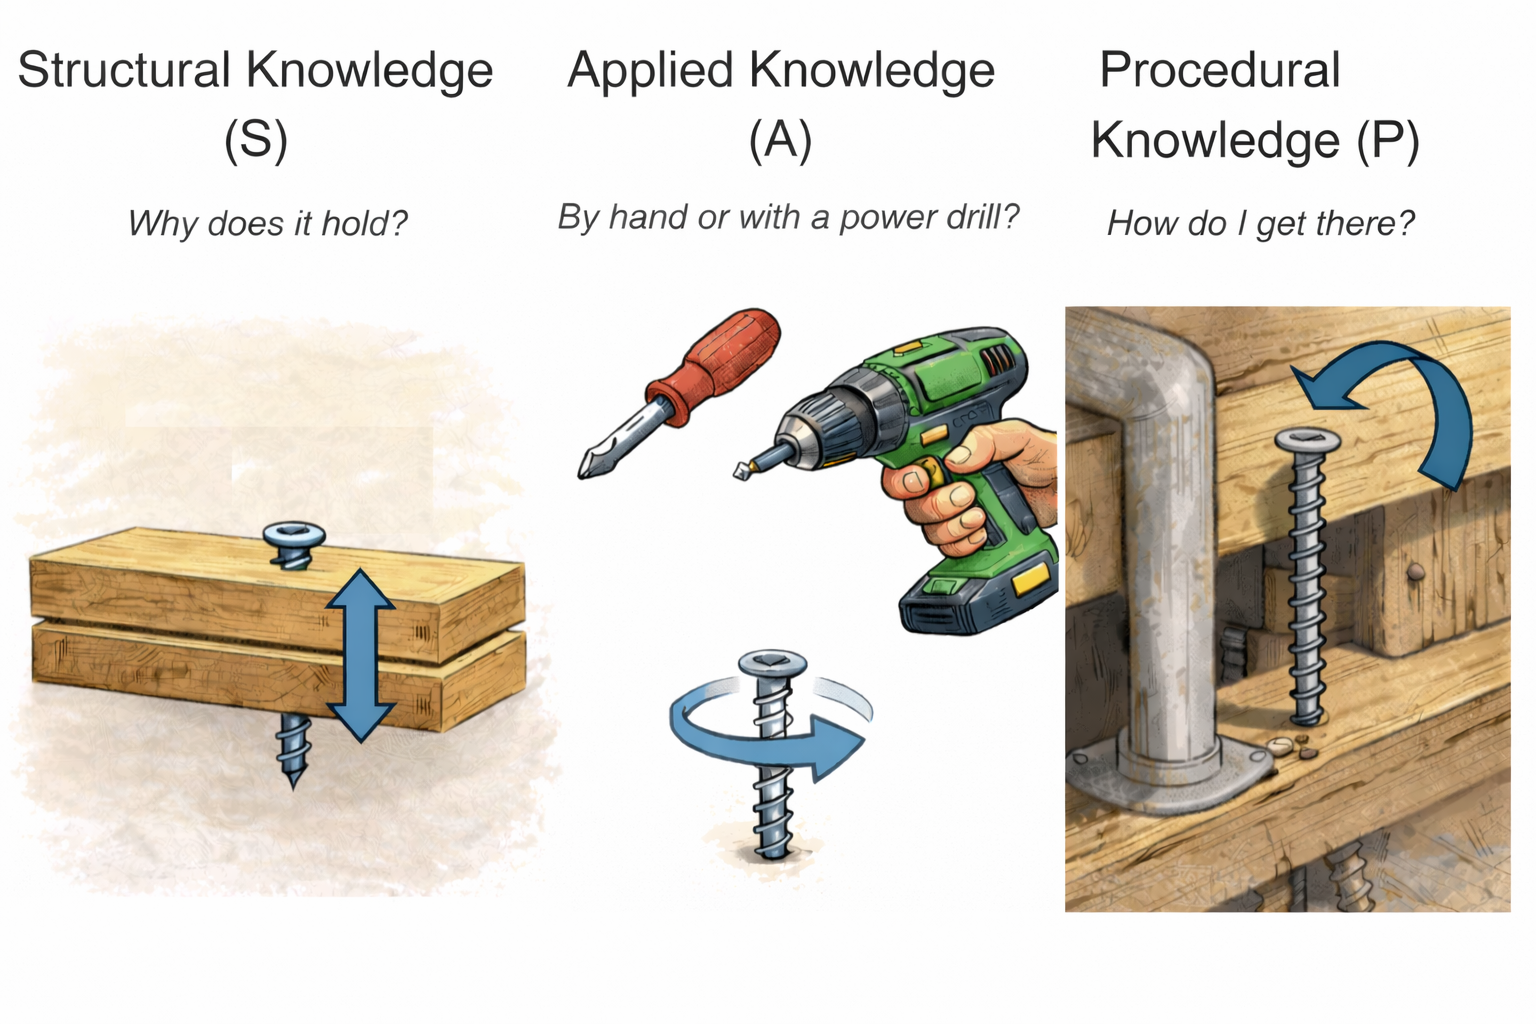
\includegraphics[width=0.6\linewidth]{screwexample.png}
\caption{Metaphor used to communicate the knowledge-marker concept.}
\label{fig:knowledge-markers-metaphor}
\end{figure}

The key message is that tools can increasingly help with application. In practice, a person may tighten a screw by hand a few times and then use a power screwdriver. For learning, the analogue is that students should not tighten 10,000 screws by hand. They should understand the principle (S), implement solutions once they understand (A), and use a method to reach reliable outcomes (P). In the AI era, Structure and Procedure knowledge build durable understanding and judgement. These are the points where instructors should slow down, require explanations, and train verification.\par

\subsubsection{How instructors use the markers}
For instructors, the markers serve as a design and analysis tool. Existing materials can be annotated, imbalances between knowledge types can be identified, and course sequences can be restructured.\par

In marked materials, (A)/(S)/(P) labels should not be placed only on parts or top-level chapters. Instead, the label should be attached to the deepest meaningful content unit in each branch. This keeps the markers useful in practice. Within a single chapter, students can switch between practicing implementation (A), clarifying mental models (S), and following a systematic procedure (P) depending on their current problem.\par

\subsubsection{How students use the markers}

The markers are intended as orientation, not as evaluation. Students can:\vspace{-2mm}
\begin{itemize}[leftmargin=*]
  \item choose an (A) unit when they want to practice and build fluency,\vspace{-1mm}
  \item switch to (S) when they notice they cannot explain what is happening,\vspace{-1mm}
  \item use (P) when tasks require a method (debugging, verifying, deciding between alternatives).
\end{itemize}

In our materials, some units additionally carry a star (e.g., (A*)). The star denotes a self-study variant: students are expected to practice these units independently, typically after lecture time has established the relevant Structure and Procedure knowledge. This makes time allocation explicit and helps balance conceptual grounding with sufficient application practice.

We actively encourage students to reflect on their methods and solutions during exercises. We use a simple self-check rule: if you cannot explain it, you do not understand it yet. When stuck, students should not only do more of the same. They should deliberately switch from (A) practice to (S) understanding or (P) procedure, such as debugging and verification. This also supports critical AI use. Students can treat AI outputs as hypotheses that must be understood (S) and verified systematically (P) before they are adopted (A).
The A/S/P labels may therefore help prevent surface learning. Without reflection and timely shifts from (A) practice to (S) understanding or (P) systematic procedure, repeated practice can become syntax pattern matching. This risk is amplified when AI can produce plausible-looking solutions instantly.






\section{Application to a Real Course}
\label{sec:case-study}

In this section, we illustrate how A/S/P markers can be used to analyse and redesign an introductory programming course. As an example, we use \emph{Programmieren} (module L1171), a compulsory first-semester course in the Bachelor's curriculum LRB at Hochschule M\"unchen University of Applied Sciences.\par
L1171 is part of the umbrella module \emph{Ingenieurinformatik} (L1170) in a non-computer-science programme. The umbrella module consists of two submodules: L1171 \emph{Programmieren} (our focus here) and L1172 \emph{Numerik f\"ur Ingenieure}. The course targets first-semester students with little or no prior programming experience. The official curriculum and syllabus are publicly available in the module handbook.\footnote{\url{https://mediapool.hm.edu/media/fk03/fk03_lokal/studierende_/modulhandbuch_archiv/lrb_1/2026_SoSe26_LRB_MHB_FKR_20260211.pdf}}\par

To improve students' learning experience, we redesign the course around live coding with minimal setup effort and a tighter coupling of theory and practice. We adopt an interactive, web-based course format that combines conceptual explanations with executable Python code cells, enabling students to learn by experimentation. As a starting point, we reuse and adapt an existing open course website \citep{ZoennchenCTBook}, which has previously been used as companion material for a ``Computational Thinking'' lecture and is available under a share-alike license that permits reuse and adaptation.\par

\subsection{Requirements for the redesign}
We derive three practical requirements from the module handbook and our teaching constraints.\par
\begin{itemize}[leftmargin=*]
  \item \textbf{R1} Curriculum focus on Application and Procedure: students should be able to develop new technical and scientific programs and assess and extend existing ones. This requires \emph{both} Application knowledge (A) (implementing solutions and applying algorithms) and Procedure knowledge (P) (selecting appropriate constructs and techniques, reasoning about program flow, and working systematically when extending or judging a program).
  \item \textbf{R2} Tight coupling of concepts and exercises: theory and exercises should be closely interleaved so that students can build understanding by applying concepts immediately in code.
  \item \textbf{R3} Time budget and scope: the contents must fit into 12 lectures plus approximately 4 hours of self-study per week over a 12-week term. This constrains how much standalone theory can be included and motivates concise explanations paired with repeated practice and procedural routines.
\end{itemize}


\subsection{Evaluating existing material}
As a first step, we use the knowledge markers to assess whether the existing materials \citep{ZoennchenCTBook} match the requirements R1 and R2. For this initial assessment, we assign one primary marker per chapter:

\begin{itemize}[leftmargin=*]
  \item Introduction: 1. Course concept; 2. What is Computational Thinking? (S); 3. History of computers and algorithms (S); 4. Why Computational Thinking? (S); 5. Let us think (P).
  \item Theory: 6. Mathematical foundations (S); 7. The digital computer (S); 8. What is information? (S); 9. Programming languages (S); 10. The art of programming (S).
  \item Python: 11. Programming in Python (A); 12. The Python ecosystem (A); 13. Basics (A); 14. Data types (basics) (S); 15. Data types (continued) (A); 16. Functions (A); 17. Control structures (A); 18. Object-oriented programming (A); 19. CPython (S).
  \item Computational Thinking in action: 20. Robot world (A); 21. Speaking in the diving bell (A); 22. Binary drawing (A); 23. Memory---everything is a list (S); 24. Name register (S).
\end{itemize}

This initial annotation highlights a pronounced split: early chapters focus on conceptual foundations, followed by application-oriented Python chapters. This violates R2 because it separates theory and practice for long stretches instead of interleaving them.\par
It also violates R1: Procedure knowledge (P) is underrepresented relative to the curriculum goal of developing, assessing, and extending programs. Finally, it violates R3: several chapters are substantial enough to fill a full lecture, which is appropriate for a comprehensive reference but too extensive for our available course time.\par
Consequently, we cannot adopt the material unchanged. We redesign it to foreground both Application (A) and Procedure (P). Structure (S) units remain concise and serve as checkpoints for application work and systematic verification.\par



\subsection{Redesigning the course}
To meet the requirements, we restructure the material around two primary emphases: application practice (A) and procedural competence (P). Structure (S) content remains concise and serves as a checkpoint for application work. We also introduce Procedure units for systematic work in software engineering, such as planning, debugging, testing, verification, and decision-making when extending or judging a program. The redesigned contents are organised into four parts (see \Cref{fig:coursestructure}). They progress from foundations to application practice and finally to the process view, that is, how software is developed:
\begin{itemize}[leftmargin=*]
  \item Foundation (\emph{Basiswissen}): shared vocabulary and a mental model of how computers represent and process information.\vspace{-1mm}
  \item Understanding Python (\emph{Python verstehen}): core concepts and background knowledge that answer typical ``why-does-this-happen?'' questions.\vspace{-1mm}
  \item Applying Python (\emph{Python anwenden}): the main focus of the course; students write and structure many small programs and implement basic algorithms.\vspace{-1mm}
  \item Case study (\emph{Fallbeispiel}): an end-to-end workflow from problem statement to planning, implementation, and interpretation of results.\vspace{-1mm}
\end{itemize}
\vspace{-1mm}


\begin{figure}[hbt!]
  \centering
  \begin{tikzpicture}[font=\small, node distance=6mm]
    \node[draw, rounded corners, align=center, inner sep=5pt, text width=2.5cm] (p2) {Part II\\Foundation\\(\emph{Basiswissen})\\about 10\%\\dominant: S};
    \node[draw, rounded corners, align=center, inner sep=5pt, text width=2.5cm, right=of p2] (p3) {Part III\\Understanding\\(\emph{Python verstehen})\\about 10\%\\dominant: S+P};
    \node[draw, rounded corners, align=center, inner sep=5pt, text width=2.5cm, right=of p3] (p4) {Part IV\\Applying\\(\emph{Python anwenden})\\about 70\%\\dominant: A+P};
    \node[draw, rounded corners, align=center, inner sep=5pt, text width=2.5cm, right=of p4] (p5) {Part V\\Case study\\(\emph{Fallbeispiel})\\about 10\%\\dominant: P+A};
  
    \draw[->, thick] (p2.east) -- (p3.west);
    \draw[->, thick] (p3.east) -- (p4.west);
    \draw[->, thick] (p4.east) -- (p5.west);
  \end{tikzpicture}
  \caption{Progression and distribution of dominant knowledge markers across course parts.}
  \label{fig:coursestructure}
  \end{figure}

In our module structure, these parts roughly correspond to a 10\%/10\%/70\%/10\% time split (foundation; Python concepts; applied practice; case study). The application-heavy phase remains practice-oriented. At the same time, Procedure knowledge is trained throughout. Students repeatedly encounter debugging and verification routines and decision points when adapting and assessing programs, not only at the end.\par
Importantly, none of the parts is meant to be purely (A), (P) or (S). Even in concept-heavy parts, we include short applied walkthroughs so that students see what a concept looks like in code (e.g., discussing control structures and data structures conceptually and then showing how their use appears in Python). Conversely, in the application-heavy part we deliberately include Structure and Procedure units to prevent rote pattern copying and to connect practice back to mental models and verification routines. The marker attached to a unit denotes its primary learning intent, not the absence of other elements.

To communicate the intended abstraction level of the four parts, we describe them as a learning journey using a driving analogy. Python is the concrete vehicle. Programming competence is the ability to drive safely and reliably toward a destination. Part~II (Foundation) establishes the basic road infrastructure and vocabulary: how a computer represents and processes information, and which constraints define what can be done. Part~III (Understanding Python) focuses on how the vehicle works. Learners build a mental model of Python's behaviour so they can explain what happens when they steer, brake, or change gears, i.e., when they use core language constructs. Part~IV (Applying Python) is driving practice. Students develop fluency by repeatedly operating the vehicle on many short routes. Part~V (Case study) is the full trip: planning a route, driving under realistic constraints, and checking safety along the way through testing, debugging, and verification. The goal is to reach the destination by method, not by accident.\par





\subsection{Implementation}
The course is implemented as open artifacts. All artifact links, archived versions, and repository entry points are provided in Appendix~\ref{app:artifacts-and-availability}.\par
We provide two main learning materials for students (see \Cref{fig:artifacts}). In both, A/S/P markers are placed in the section headlines at the finest-grained level:
\begin{itemize}[leftmargin=*]
\item An interactive learning website that contains conceptual explanations and practical exercises in Python.
\item A PDF script with aligned content; unlike the website, Python code cells are not executable.
\end{itemize}


\begin{figure}[hbt!]
  \centering
  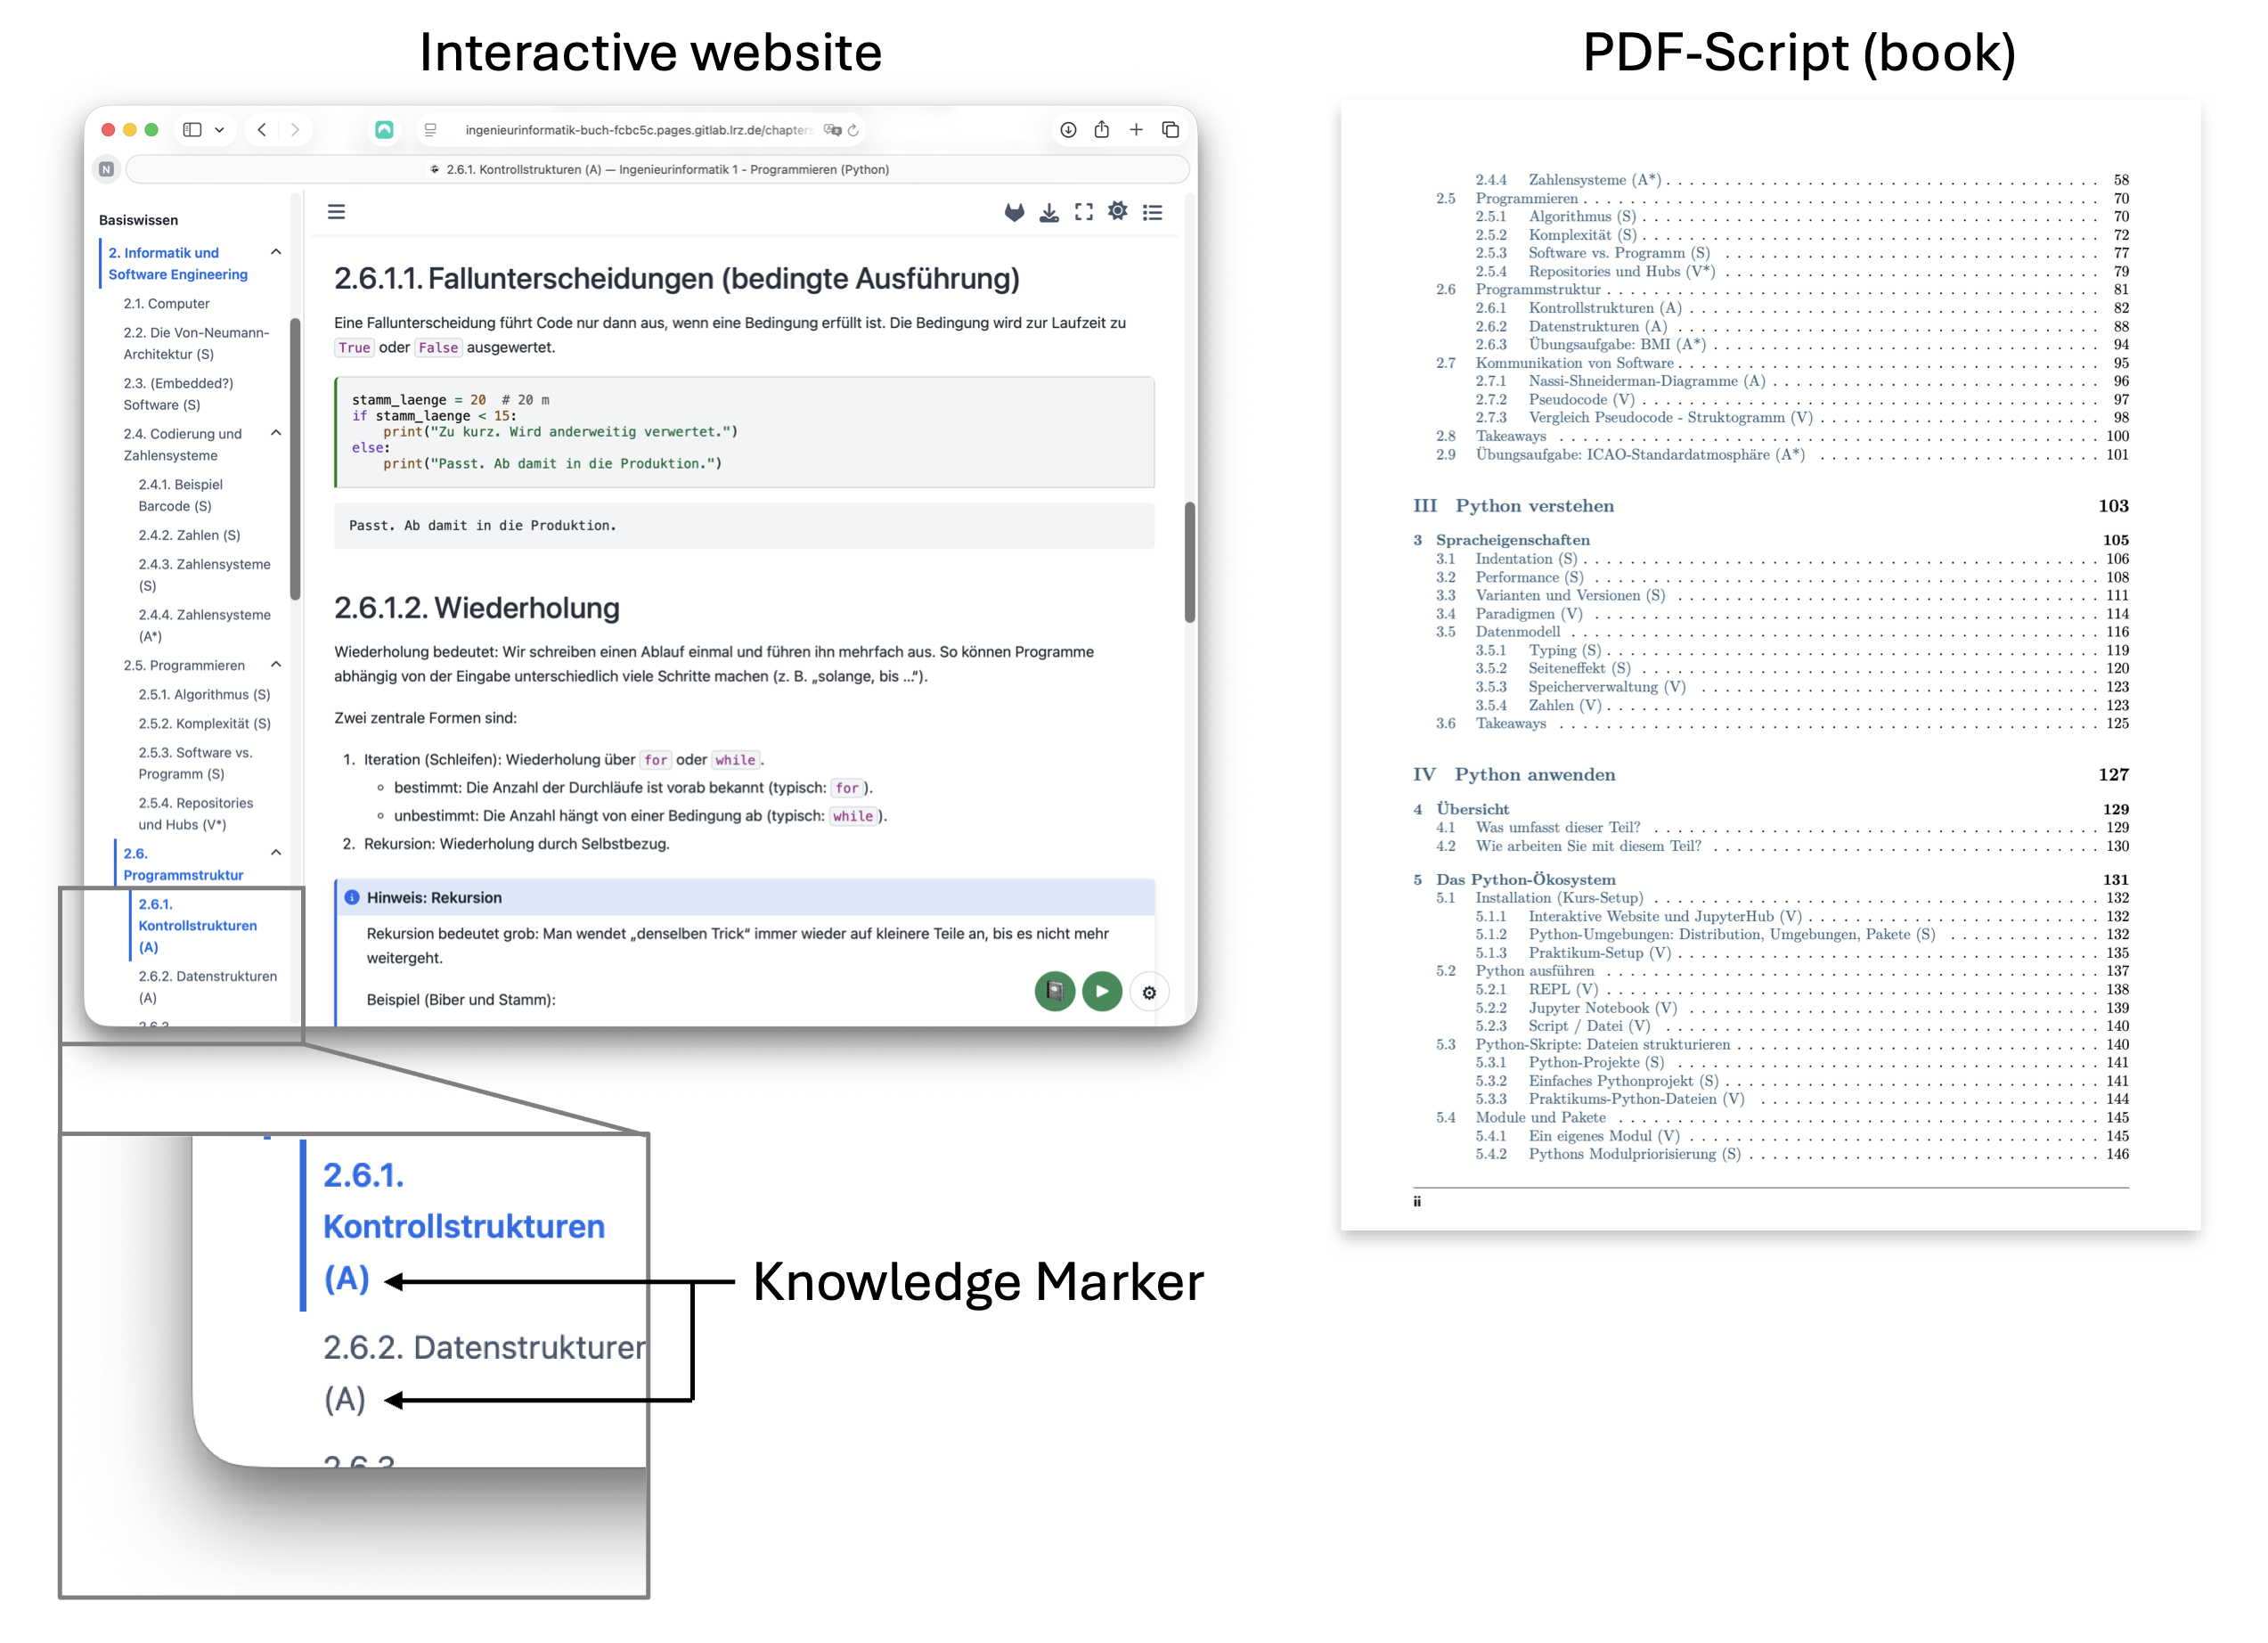
\includegraphics[width=0.9\linewidth, trim=0cm 0cm 0cm 0cm, clip]{artifacts.png}
  %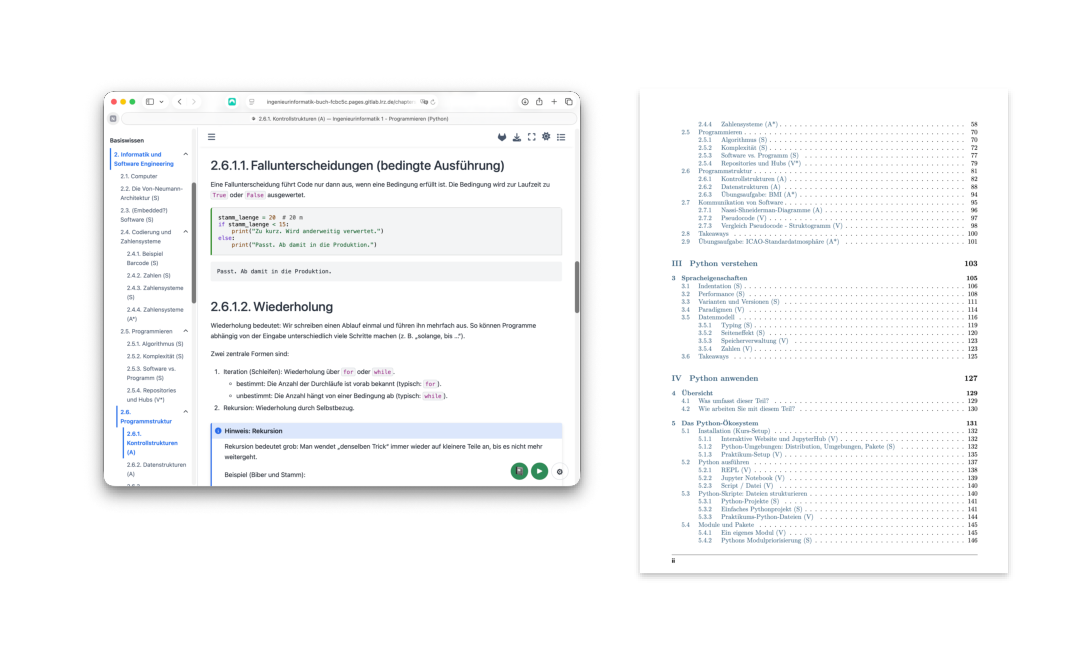
\includegraphics[width=0.98\linewidth, trim=1cm 1cm 1cm 1cm, clip]{artifacts.pdf}
  \caption{The two learning artifacts students work with: the interactive website (left) and the PDF script (right). The contents are aligned, but the website also lets students execute Python code in interactive code cells. Knowledge markers are assigned at fine granularity and are visible in the table of contents (left and right).}
  \label{fig:artifacts}
  \end{figure}


The website lets students execute Python code cells in the browser. This lowers setup effort and supports rapid hypothesis testing. Learners can run, vary, and verify examples instead of treating code as static text. The PDF script is a stable, offline-friendly reference. It mirrors the website structure and preserves the course as a citable artifact, for example for exam preparation and long-term reuse. In addition, Jupyter Notebooks are provided for environments where students work locally or in managed notebook services.\par




In addition to the A/S/P markers, the course concept addresses a practical constraint: students may use general-purpose LLM tools (e.g., ChatGPT) with or without explicit permission. Related work suggests that learning outcomes depend strongly on usage patterns and constraints. Unrestricted use can increase overreliance. Requiring learners to state intentions and explanations can reduce this risk \citep{Sankaranarayanan2026EpistemicDebt}. We therefore provide optional usage guidance. Students decide whether and how to use AI. If they use it, the guidance asks them to seek explanation and systematic verification rather than finished solutions.\par
To operationalise this intended stance (AI as a learning coach rather than a solution outsource), the materials include the following prompt template:
\begin{quote}
\small
\begin{verbatim}
I need to write a Python program that solves:
<TASK>

Please do not give me finished source code.
Help me step by step with method:
- Which requirement questions and boundary conditions should I clarify?
- What are the program inputs/outputs (file, console, API)?
- Which data structures and control structures fit?
- Which libraries could be relevant (examples only)?
- How can I test it (small tests, edge cases)?
\end{verbatim}
\end{quote}



\subsection{Descriptive material analysis}
\label{sec:evaluation}
We use the knowledge markers to analyse whether the redesign aligns with the module-handbook emphasis on both application and procedure. This is a descriptive material analysis. It does not measure student learning outcomes, motivation, or transfer. Instead, it checks whether the designed course materials visibly reflect the intended balance of Application, Structure, and Procedure knowledge. For this purpose, the marker labels analysed in this section are not a direct copy of the labels in the original teaching artifacts. They were created specifically for the paper analysis. The distinction is important because the two versions serve different purposes: the teaching artifacts are course materials for students, whereas the cleaned analysis version is a reproducible A/S/P analysis artifact.\par

Label differences between the teaching artifacts and the cleaned analysis version are therefore expected rather than errors. The teaching artifacts had already been generated while the A/S/P assignment system was still being refined. At that stage, the final decision tree was not yet fully worked out, some labels were missing, and teaching-specific variants such as \(A^*\) were still present. 
For the paper analysis, we therefore recoded the material in a separate cleaned analysis version. In that version, the table of contents defines the units to be counted, the final decision tree is applied uniformly, and each row receives exactly one value so that page-count and section-count distributions can be computed. 
Teaching-specific variants are normalised (e.g., \(A^*\) is counted as (A)), purely organisational units are marked with \texttt{-}, and higher-level sections are labelled when they contribute conceptual structure, context, or orientation. 
The cleaned labels provide a consistent coding of the material for the descriptive analysis reported here. 
A detailed comparison of the two versions is provided in Appendix~\ref{app:teaching-vs-analysis-version}.\par

The human labels are the primary analysis basis. As a consistency check, we additionally compared them with labels generated by a large language model using the file-based procedure described in Section~\ref{sec:llm-assignment}. The LLM assigned the same label as the human rater for 156 of 199 units (78.4\,\%). This comparison is not a formal inter-rater reliability study because the second rater is a model, not an independent human coder. It is used as a practical check for ambiguous units. Differences are treated as indicators of interpretive borderline cases rather than as automatic errors. The complete comparison table is provided as supplementary material, and a summary is given in Appendix~\ref{app:llm-comparison}.\par

To assess whether the material design reflects the intended shift toward (A) while retaining (S) and (P), we use two complementary measures:
\begin{itemize}[leftmargin=*]
  \item \textbf{Page-count distribution}: the number of pages labelled (A), (S), (P), or \texttt{-}. This is a proxy for material allocation, i.e., how much space the materials allocate to each type.
  \item \textbf{Section-count distribution}: the number of listed units labelled (A), (S), (P), or \texttt{-}. This approximates structural emphasis, i.e., how many distinct ideas/checkpoints the course comprises.
\end{itemize}
\vspace{-1mm}

We compute both measures per course part to examine whether the intended trajectory across parts is reflected in the materials. Counts are derived from the table of contents of the clean printable PDF script (version 2.6.8); page counts are approximate and may vary slightly with PDF build settings. The distributions for the human labels are shown in \Cref{fig:marker-distributions}.\par

\begin{figure}[hbt!]
  \centering
  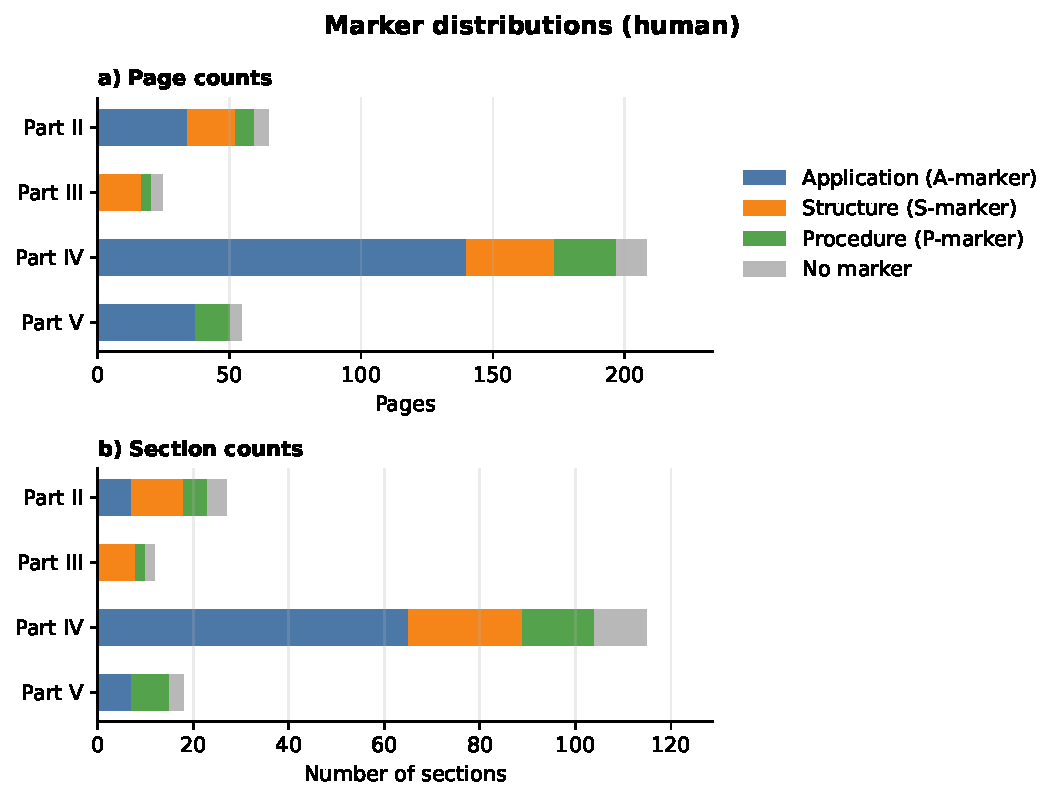
\includegraphics[width=0.9\linewidth]{marker_distributions_human.pdf}
  \caption{Knowledge-marker distributions across course parts based on the cleaned analysis version and human labels. Page counts approximate quantitative emphasis; section counts approximate structural emphasis.}
  \label{fig:marker-distributions}
\end{figure}

The two measures make the redesign outcome visible in complementary ways. The \emph{page-count distribution} captures material allocation: Part~IV (Applying Python) dominates the materials with 208.5 pages in the analysed table-of-contents units. Of these, 140 pages are labelled (A), 33.5 pages (S), 23.5 pages (P), and 11.5 pages \texttt{-}. Thus, the main practice phase is clearly application-heavy, as required by the module handbook, while still reserving substantial space for conceptual checkpoints and systematic working practices. At the level of material design, this aligns with R1.\par

The \emph{section-count distribution} answers a different question: how often do students encounter each learning emphasis, independent of unit length? In Part~IV, the 65 application-oriented units are interleaved with 24 structure-oriented and 15 procedure-oriented units. This indicates that (S) and (P) are not confined to an introductory block. They recur throughout the main practice phase, where students are most likely to rely on pattern matching or accept AI-generated solutions without verification.\par

Across parts, the distributions reflect the intended learning trajectory. Part~II (Foundation) is mixed, with (A), (S), and (P) all present. Part~III (Understanding Python) concentrates on (S)/(P), with no application-labelled unit in the analysed table. Part~V (Case study) returns to application while increasing the relative importance of procedure: 8 of 18 listed units and 13.5 of 54.5 pages are labelled (P). This is consistent with an end-to-end workflow where planning, decomposition, testing, and verification matter alongside writing code.\par
At the same time, the distributions show that theory and practice are not separated by part boundaries. Each substantive part contains a mix of learning emphases. At the level of material design, this aligns with R2 because conceptual checkpoints and procedural routines are interleaved with application work. The manageability of the overall scope is not directly visible from these distributions. At chapter level, the script comprises ten main chapters; manageability in teaching practice will be assessed in the course iteration starting in Summer Semester 2026.\par






\section{Discussion}
\label{sec:discussion}
Generative AI changes the design problem of programming education. When students can generate plausible code with little effort, course design can no longer rely on code production alone as evidence of learning. The central question is therefore not only whether AI should be allowed. It is also whether existing course contents still serve learning when implementation can be partly automated. Instructors need a way to judge what a unit is for: Does it train implementation fluency, build a transferable mental model, or develop systematic procedures for debugging, testing, and verification? Without explicit labels for these purposes, instructors have little support for deciding which materials should be kept, reduced, moved to self-study, redesigned, or strengthened in an LLM-shaped learning environment.\par

Knowledge markers address this problem by providing a simple middle layer between learning theory, course design, and AI-supported practice. The A/S/P distinction does not replace detailed taxonomies or empirical evaluation. Instead, it makes the object of course analysis visible at the level where instructors and students actually work: individual course units. Its primary use is practical course analysis and redesign. Instructors can inspect what a course asks students to do. They can check whether application-heavy parts include enough conceptual checkpoints and procedural routines. They can also decide where AI use may accelerate work without replacing the intended learning. For students, the same labels clarify how they should approach a unit and when they should switch from implementation practice to explanation or verification. As an additional benefit, this explicit labelling can also make empirical studies easier to interpret and compare. Interventions can then be described by their targeted knowledge emphases, not only by the tool that was used.\par

The case study illustrates how the markers can be used as a practical design instrument. The module handbook requires students not only to write programs, but also to assess, extend, and work systematically with them. The initial annotation of existing material made visible that conceptual foundations and application-oriented Python chapters were separated, while Procedure knowledge was underrepresented. This diagnosis directly informed the redesign: application practice remains dominant, but Structure and Procedure units are deliberately interleaved so that students repeatedly encounter explanation, debugging, testing, and verification while they practise implementation.\par

The marker distributions make the redesign visible at the material level. Page counts approximate how much material is allocated to each knowledge emphasis. Section counts show how frequently learners encounter each intent. In the redesigned course, the main practice phase is clearly application-heavy, as required by the module context. It also contains recurring Structure and Procedure checkpoints. This matters in the AI era because these checkpoints are where students slow down, explain behaviour, test assumptions, and verify results instead of merely accepting generated code.\par

The assignment procedure itself is part of the contribution. We show that a human rater can assign the markers using the definitions and decision tree. We also demonstrate LLM-supported assignment using the same rules. The LLM labels are not treated as ground truth or as a replacement for instructor judgement. Instead, they provide an additional label proposal. Agreement indicates straightforward cases. Disagreement highlights ambiguous or mixed-emphasis units where the intended learning focus may need clearer communication. This matters for reuse because a course-level concept is only practical if people can apply it consistently enough and if tools can help when materials become large.\par

For instructors, the concept is useful for both planning and revision. During planning, markers help decide where conceptual explanations, implementation practice, and systematic procedures should be placed. During revision, marker distributions and sequences reveal concrete design problems. A course may contain long stretches without verification practice. Theory may be concentrated too early. Application exercises may lack conceptual support. Because the labels are simple, this analysis can be performed without specialised didactic training and without committing to a specific AI tool, platform, or assessment regime.\par

For students, the markers provide orientation for learning behaviour. They indicate whether the current task asks them primarily to implement, to understand, or to proceed methodically. This gives students a simple learning strategy. When implementation practice fails or becomes superficial, they should not only do more of the same. They should switch to explaining the underlying structure or applying a systematic debugging and verification method. Optional AI-usage guidance can then follow the same logic. AI may help with implementation, explanation, or reflection, but generated output still has to be understood and verified.\par

The concept also reframes AI policy discussions. Whether AI is allowed, restricted, or actively integrated is an important institutional decision, but it does not by itself define what students should learn. A/S/P markers make the learning demand explicit before tool decisions are made. If AI is allowed, the markers clarify where automation may accelerate application work and where learners must still build understanding and judgement. If AI is restricted, the same markers still structure the course around implementation, conceptual understanding, and systematic procedure.\par

The limitations of the approach follow from its intended simplicity. A/S/P labels are coarse and identify the primary learning emphasis of a unit, not all knowledge involved. Borderline cases require judgement, and different raters may classify mixed units differently. The comparison between human and LLM labels makes this interpretive component visible rather than hiding it, but it is not a substitute for an inter-rater reliability study with independent human coders. In this paper, the marker distributions provide a descriptive analysis of course alignment rather than a measurement of student learning outcomes. Page counts are also only a proxy for material allocation; they do not directly measure study time or cognitive effort. This descriptive step is useful in its own right for course design and revision; it also prepares later empirical work by making the designed learning emphases explicit and reproducible.\par

Overall, the contribution of knowledge markers is to make programming course design more transparent under conditions of increasing automation. The concept helps instructors analyse whether course contents still contribute to learning in the age of LLMs. It also helps them redesign the balance between application, structure, and procedure, document what a course asks students to learn, and decide where AI support is appropriate. Explanation and verification can then remain central where they are needed. The markers also help students adjust their learning strategies. Only after this design layer is explicit can empirical work compare AI-supported interventions more precisely. The open teaching artifacts demonstrate that the approach can be implemented in a real course without requiring a dedicated AI system or a complex didactic framework.\par



\section{Conclusion}
This paper introduced knowledge markers (A/S/P) as an AI-agnostic concept for structuring and analysing programming education. The markers distinguish whether a learning unit primarily targets Application knowledge, Structure knowledge, or Procedure knowledge. This simple distinction makes learning intent explicit at the level of concrete course units and helps instructors decide whether course contents still serve learning in a context where implementation can be partly automated. It also supports the redesign of materials in which implementation practice, conceptual understanding, and systematic verification are deliberately balanced.\par

The contribution is particularly relevant in the context of generative AI. When code production becomes easy to automate, it becomes harder to infer what students have actually learned from the programs they submit. Knowledge markers address this challenge by making visible what kind of knowledge a task is meant to develop and what kind of student activity should therefore be protected or supported. This enables instructors to analyse existing materials, identify parts that overemphasise automatable routines, and strengthen units that build understanding, judgement, and verification.\par

We demonstrated the concept in a real introductory programming course for a non-computer-science programme. The markers were used to analyse existing material, guide a redesign, communicate learning intent to students, and summarise the resulting course structure through page-count and section-count distributions. We also showed that marker assignment can be performed manually and supported by LLMs using the same rules. Disagreements serve as useful signals for ambiguous units. The open artifacts show how the concept can be embedded in an interactive website, a PDF script, and accompanying notebooks.\par

Future work can build on this explicit course-design layer. Empirical studies can investigate how students use the markers for navigation, help-seeking, AI interaction, explanation, debugging, and verification. Reliability studies with independent human raters can also test how consistently the markers are assigned across courses and institutions. Because the intended knowledge emphases are explicit, such studies can be designed and compared more precisely. In this sense, knowledge markers are first a design and analysis layer for course contents. Their value for empirical comparability follows from this primary role: they clarify what was designed, what students were asked to learn, and what an AI-supported intervention is expected to affect.\par


\bibliographystyle{unsrtnat}
\bibliography{references}  %%% Uncomment this line and comment out the ``thebibliography'' section below to use the external .bib file (using bibtex) .


\appendix
\section{Supplements}
\label{app:artifacts-and-availability}

The current live version of the interactive course website is available at

\url{https://ingenieurinformatik-buch-fcbc5c.pages.gitlab.lrz.de/intro.html}

Because this live website may change over time, we recommend citing the archived version used for this paper (see below).

The source material from which the website is deployed is linked within the website. Direct link: \url{https://gitlab.lrz.de/fk03ingenieurinformatik/Ingenieurinformatik-buch}. The technical documentation can be found here: \url{https://gitlab.lrz.de/fk03ingenieurinformatik/Ingenieurinformatik-buch/-/tree/master/_docs}


The teaching artifacts referred to in this paper are archived on Zenodo:\par
\begin{itemize}[leftmargin=*]
  \item Interactive website (archived): \href{https://doi.org/10.5281/zenodo.19032453}{10.5281/zenodo.19032453}\vspace{-1mm}
  \item PDF script (archived): \href{https://doi.org/10.5281/zenodo.19033460}{10.5281/zenodo.19033460}\vspace{-1mm}
  \item Source repository (archived): \href{https://doi.org/10.5281/zenodo.19032388}{10.5281/zenodo.19032388}
\end{itemize}
\vspace{-1mm}
All archived items are cross-linked to show dependencies.

In Section~\ref{sec:evaluation}, marker distributions are used to describe the redesigned course structure. Page counts approximate material allocation. Section counts approximate how frequently students encounter each learning emphasis. The following Zenodo archives provide the data and scripts behind that analysis:\par
\begin{itemize}[leftmargin=*]
  \item \textbf{A/S/P analysis supplement}: \href{https://doi.org/10.5281/zenodo.19790470}{10.5281/zenodo.19790470}. This dataset contains the analysis based on the cleaned PDF script and its table of contents: the human and LLM label-assignment input packages, marker assignment results, merged label table, marker-distribution summaries, generated plots, and analysis scripts.\vspace{-1mm}
  \item \textbf{Source/build archive}: \href{https://doi.org/10.5281/zenodo.19790605}{10.5281/zenodo.19790605}. This archive contains the source repository version under the tag \texttt{supplements-paper} and documents the build pipeline used to create the cleaned PDF script and table of contents.
\end{itemize}
\vspace{-1mm}
These archives serve different purposes. The archived teaching artifacts document the course as implemented for students. The A/S/P analysis supplement documents the cleaned analysis version used for the descriptive analysis. For that analysis, we generated marker-assignment tables from the table of contents of the cleaned PDF script. The human rater and the LLM then assigned exactly one label to each listed unit using the definition and decision criteria introduced in Section~\ref{sec:asv}. The human labels form the basis for the marker distributions reported in this paper.

\subsection{Teaching artifacts and cleaned analysis version}
\label{app:teaching-vs-analysis-version}

\Cref{tab:teaching-vs-analysis-version} summarises why labels in the teaching artifacts can differ from the labels in the cleaned analysis version used for the descriptive analysis.

\begin{table}[hbt!]
  \centering
  \small
  \caption{Difference between the original teaching artifacts and the cleaned analysis version used for the descriptive analysis.}
  \label{tab:teaching-vs-analysis-version}
  \begin{tabularx}{\linewidth}{@{}lXX@{}}
  \toprule
  \textbf{Aspect} & \textbf{Teaching artifacts} & \textbf{Cleaned analysis version} \\
  \midrule
  Purpose & Course material generated while the A/S/P system was still being refined & Reproducible A/S/P analysis for this paper \\
  Decision tree & Not yet fully worked out when some labels were added & Final decision tree applied systematically to all listed units \\
  Label coverage & Some units were unlabelled or labelled inconsistently & Every listed unit receives exactly one analysis label \\
  Granularity & Mostly labels the finest-grained learning units & Labels parts, chapters, sections, and units when they carry an identifiable learning emphasis \\
  Marker set & Includes teaching-specific variants such as \(A^*\) for self-study & Uses only (A), (S), (P), and \texttt{-} \\
  \bottomrule
  \end{tabularx}
\end{table}

\subsection{License and reuse}
The teaching artifacts (website, PDF script, and notebooks) are released as open educational resources under a Creative Commons Attribution-ShareAlike license (CC BY-SA 4.0). The Zenodo archives provide stable references for citation and reuse.\par

\subsection{Illustrations}
Some illustrative figures in the teaching materials were created with generative AI for didactic visualization. They contain no empirical measurements or study data.\par

\subsection{Automatically generated labels using LLMs}
\label{app:llm-comparison}

The LLM-based labelling was performed with the same marker definition and decision process used for the human labelling, but the decision tree was supplied in a different representation: the human rater received it as an image, while the LLM received the corresponding textual TikZ source. The LLM input package consisted of the marker definition, this textual TikZ decision tree, the clean PDF script, and the Markdown marker-assignment table generated from the script's table of contents. The model was instructed to assign exactly one of (A), (S), (P), or \texttt{-} to each unit and to modify only the LLM-label column. The exact prompts and interaction are documented in the supplement transcript.\par

For the reported run, the model used for label assignment was GPT-5.5 in Cursor. The LLM labels matched the human labels for 156 of 199 units (78.4\,\%); 43 units differed (21.6\,\%). Differences were distributed similarly across hierarchy levels: 23 of 113 subsections differed (20.4\,\%), and 20 of 86 non-subsection units differed (23.3\,\%). The most frequent differences were \texttt{P -> S} (10 cases), \texttt{- -> S} (7 cases), \texttt{A -> S} (7 cases), and \texttt{S -> A} (6 cases). We interpret these differences as useful signals for borderline or mixed-emphasis units, not as a replacement for instructor judgement. The full comparison table, generated plots, and transcript of the LLM labelling run are included in the Zenodo supplement.

\section{Remarks}
Generative AI (ChatGPT, version 5.2) was used as a writing assistant to improve language quality (reformulation of sentences, grammar, and spelling). The tool was not used to generate new scientific claims or results.
\end{document}

